\section{The Crisis Producing Place}

In the previous books we explained the distributions with worked-out examples. Now in this book we will further clarify other powerful places and the keys which unlock the distributions of the stars.

With this having been established, it is necessary to prove by experience <the effectiveness of> still another place which I will demonstrate most abundantly: this is the Crisis-Producing Place\footnote{Schmidt calls it the Lot of Accusation (VRSV p.1). In Paulus, one of its names is the Accusative Place (PAG p.159).}, the place causative of terrors, dangers, and chains. Consequently this place is strong; for day births it is found by determining the distance from \Saturn\, to \Mars\, (for night births, from \Mars\, to \Saturn), then measuring the same distance from the Ascendant\footnote{\textsc{Riley:}others measure the distance from Mercury. - marginal note.}.

It will be necessary to examine the location of this place to see if the
sign of a malefic, or malefics themselves, are in conjunction or aspect. If they are, the nativities will be precarious, endangered, and easily destroyed. The nature of each star and sign will cause the particular type <of trouble>. Benefics in conjunction or aspect will cause a lessening of the evil or an escape from crises.

It has seemed best to use the place in this way: if the \Sun\, or \Moon\, is found to be \Sextile\, to \Saturn\, or \Mars\, (calculating by signs), the nativity will be at risk and subject to crises, particularly in the similar degrees/within 70\deg and in the listening signs. This is especially true at the time when one of the stars is making a transmission into the configuration described above. 

For example: if the \Sun\, transmits to \Saturn\,
or the \Moon\, to \Mars\,, or if \Saturn\, or \Mars\, transmits to the \Sun\, or \Moon\,, and if neither is at the same place, but one is \Sextile\, and the other is making the transmission or reception into the configuration described
above from a position \Square,\textbf{/209K/} \Trine, in \Opposition, or turned away—under these circumstances the nativity will be disturbed, will be involved in defense speeches, imprisonment, custody, or will have suspicions and crises \textbf{/199P/} about such matters and will live with a bad conscience. But if a benefic is in conjunction with any of these stars or is in an appropriate aspect, the nativity will have a respite from terrors and dangers or a change to the better, but it will not continue to be undisturbed. 

If the configuration happens to be afflicted and has no benefic in aspect, the native will be convicted and will come into chains,
imprisonment, or custody. 

If, with this configuration prevailing, the basis of the nativity is found to be great, at that time the native must have a care for his rank and livelihood: he will experience accusation and betrayal; he will defend himself before the authorities or the king—if not himself, then someone else—so that the terror and anguish <of this configuration> might be fulfilled. So great is this Place’s power!

The full effects of the crisis (imprisonment and ruin) will come to pass if the overall and the yearly chronocrators take effect at the same time. The distribution using the cyclical chronocratorships will bring terrors and misery. If an infant nativity has this configuration, it will be necessary to forecast anxiety for the father or mother—or for the master, if the nativity is that of a slave. Note that some men, even while infants, come into imprisonment or confinement and spend their lives in such places. If some benefic is in transit or in aspect with this place at such times, a respite or relief from evil will occur; if a malefic is there, worse will occur; if a benefic and a malefic are there, good and bad will occur. In addition, if malefics are found in \Opposition\, or \Square\, with the \Sun\, or the \Moon, they bring anxieties and imprisonment.

If the nativity is found to be helped in some way by an aspect of benefics or by its general basis, with the result that there is no imprisonment, then there will be some figurative type of imprisonment or condemnation: military service, custodianship, debts, loans, to be assigned to convict-duty and to be put in charge of them, or (as often happens to many) to be required to do attendance because of the law or business. Some are fated to have unwanted experiences and to be unable to act as they desire. Some seem to be under the power of others; \textbf{/210K/} even though they are free, they are punished by a bad conscience. Some travel abroad or sail, and are held somewhere on an island or in deserted places, or they do service in temples or sacred places. Occasionally they are confined by recurrent diseases or by epilepsy, fits, spells, blindness, the ague, and syndromes such as these. 

It is necessary to make a careful decision about these places, \textbf{/200P/} whether the “confinement” will be only figurative, or will be literal and involve some damaging accusation.

\newpage

\begin{wrapfigure}[14]{R}{7cm}
\centering
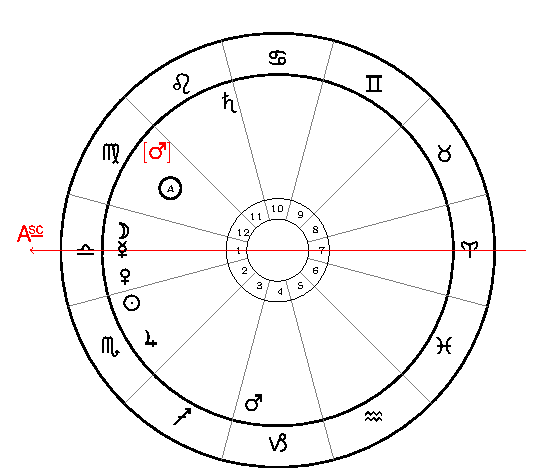
\includegraphics[width=.68\textwidth]{charts/5_01_1}
\caption{Chart 53 [V.1, GH L121]}
\label{fig:chart53}
\end{wrapfigure}

For example: \Sun, \Jupiter\, in \Scorpio, \Moon, \Mercury, \Venus, Ascendant in \Libra, \Saturn\, in \Leo,
\Mars\, in \Capricorn. Both malefics were \Sextile\, to the \Sun\, and \Moon\footnote{\textit{Greek Horoscopes} dates the chart to October 27, 121 with all planets except \Mars\, in agreement stating ``one must assume that the position of Mars is mistakenly given as Capricorn, instead of Virgo, probably on the basis of a misreading of the two symbols, which look often very similar'' (p.118)}. 

If the luminaries had lacked the presence of benefics, it would have been possible to forecast imprisonment. As it was, the configuration was magnificent and noteworthy. The native, a soldier, in his 35th year was in charge of prisoners and a prison. He fell in love with a woman in prison, was troubled by an accusation on her account, had expenses, but avoided the danger. At the same time he captured and bound a fugitive slave.

\begin{mdframed}[backgroundcolor=cyan!5]
\scriptsize
The Lot of Accusation, in a night chart, is: from \Mars\, to \Saturn, counting in the order of the signs, projected from the Ascendant which places it in \Virgo, the 12th of imprisonment, with \Mars\, (according to the \textsl{Greek Horoscopes} and the Schmidt translation placement).

The 35th year / 12 = 2 with 11 left over.  The \Sun\, and \Mars\, are 11 signs apart as are the \Moon\, and \Saturn.  The \Moon\, is with \Venus\, (woman) and \Mercury\, (ruling the Lot of Accusation) stands between them with \Venus\, in her own domicile prevailing (?). The \Sun\, is with \Jupiter\, in the 2nd house (income) and rules the 6th of slaves; he wards of real harm.
\end{mdframed}

\newpage

